\chapter{GINA Features}

The current version of GINA is a graphical user interface (GUI) program that was designed in Qt Creator on a Linux computer. Upon an initial run of GINA, there are default values filled out in every required field so that the user can generate an analysis and get an example of what GINA will provide.

\section{User Interface}

\begin{figure}[h!]
	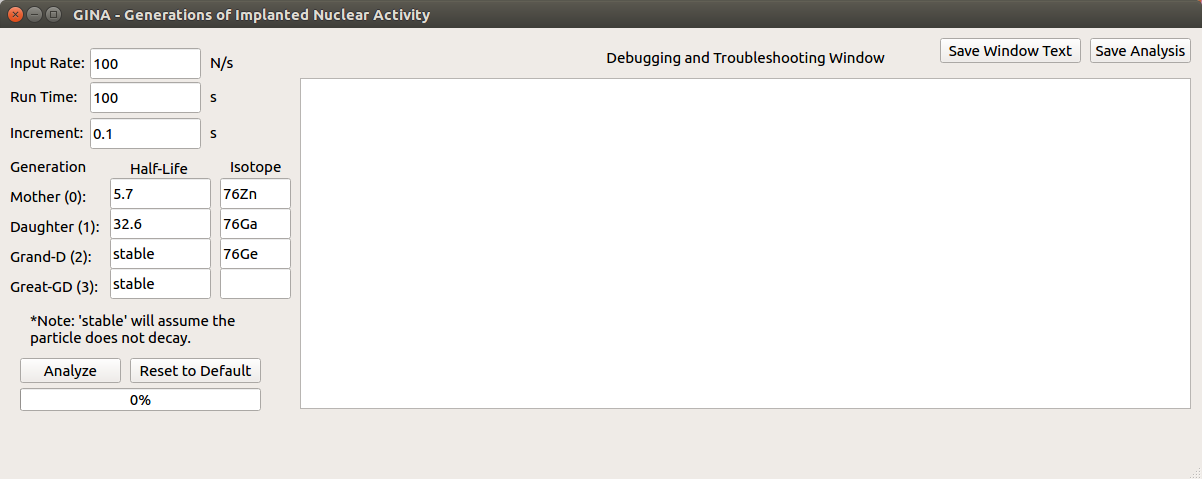
\includegraphics[scale =0.5]{./Images/GINAwindow.png}
	\caption{An example of what the GINA GUI looks like when first ran.}
	\label{fig:gui}
\end{figure}

The GINA GUI contains numerous small text fields for user input. These are all labeled appropriately. These include input rate, run time, increment, half-lives, and isotope labels and can be seen on the left side in figure \ref{fig:gui}.
\begin{itemize}
	\item Input rate - This is the rate at which radioactive isotopes are implanted onto a portion of the tape. This will not change the final results other than in magnitude.
	\item Run time - This determines the time frame that the program will run it's calculations for. It also determines the maximum x-axis values for the plots that can be generated.
	\item Increment - This determines the time increment between each value that is calculated by the program. For more accurate results (especially when dealing with isotopes with very short half lives), a short increment time is needed. The shorter the increment time, the more calculations are needed to be done by the program and thus the longer it will take to run it. Due to the process by which GINA performs all of the calculations, the accuracy of the data is also increased with a smaller increment size, though it does become negligible at sufficiently small increment sizes.
	\item Half-lives - These are the half lives of an isotope.
	\item Isotope label - These are the labels of which isotope corresponds to which half-life.
\end{itemize}

\textit{This section is still under construction...}

\section{Analysis and Analysis Text}

\textit{This section is still under construction...}

\section{User Inputs}

\textit{This section is still under construction...}

\section{Graphs and Graph Settings}

\textit{This section is still under construction...}

\begin{figure}[h!]
	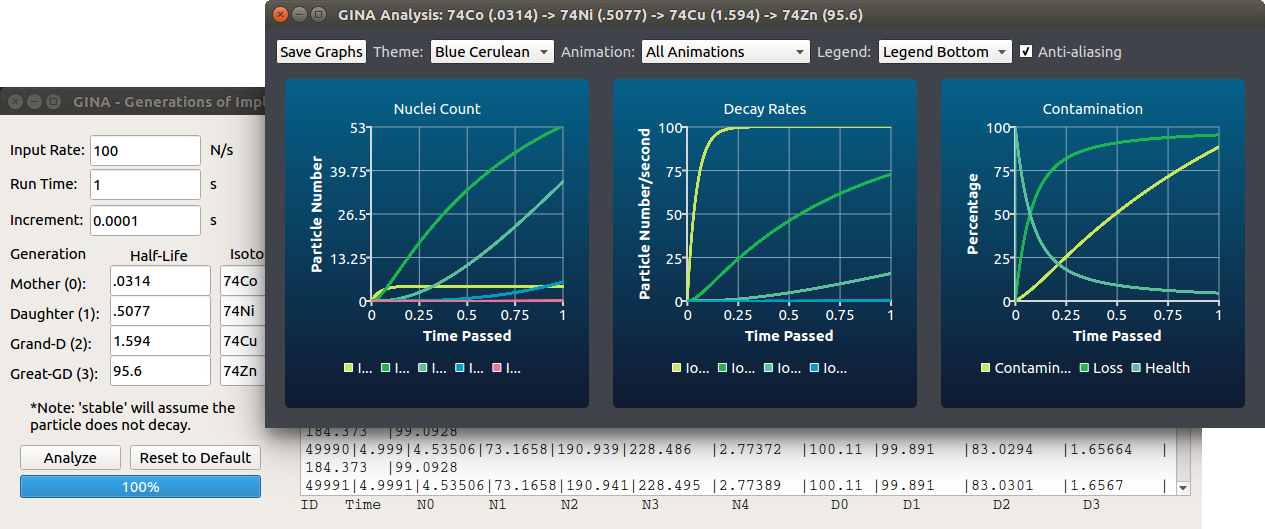
\includegraphics[scale =0.475]{./Images/GINAexample.png}
	\caption{An example of what the GINA graphs looks like when analysis is first ran.}
	\label{fig:graphs}
\end{figure}

\section{Advanced Options}

\textit{This section is still under construction...}